\documentclass[user_manual.tex]{subfiles}
\begin{document}

%Inicio de la introducción
\chapter{Introducción}

El presente manual de usuario tiene como propósito ser una guía clara y específica para garantizar el uso y funcionamiento
óptimo de Justina ``el robot de servicio'', resolver las dudas más comunes de esta, así como el desarrollo de una replica
para la investigación sobre los robots de servicio.\\
\\
Comprende de la descripción general de Justina, así como de: el hardware empleado en ésta y, el software desarrollado para su
funcionamiento.\\
\\
Contempla todo lo relacionado al hardware empleado (datasheet), así como las ligas para ver especificaciones más avanzadas de 
este, son dados para el lector interesado en una explicación más detallada. También, este documento contiene los algoritmos
creados por los desarrolladores del laboratorio de Biorobotics. Para cada modulo está incluida una breve descripción del algoritmo,
técnicas o enfoques usados para el diseño.\\
\\
Cabe señalar, que, este documento esta sujeto a actualizaciones conforme sean requeridas por actualizaciones en Justina.\\
\\
El robot de servicio Justina fue diseñado en el laboratorio Biorobotics, de la facultad de ingeniería de la UNAM.\\
\\
En la figura \ref{fig:introduction:Justina} se muestra el robot de servicio Justina.

%Figura 1.1 de Justina
\begin{figure}[H]
\centering
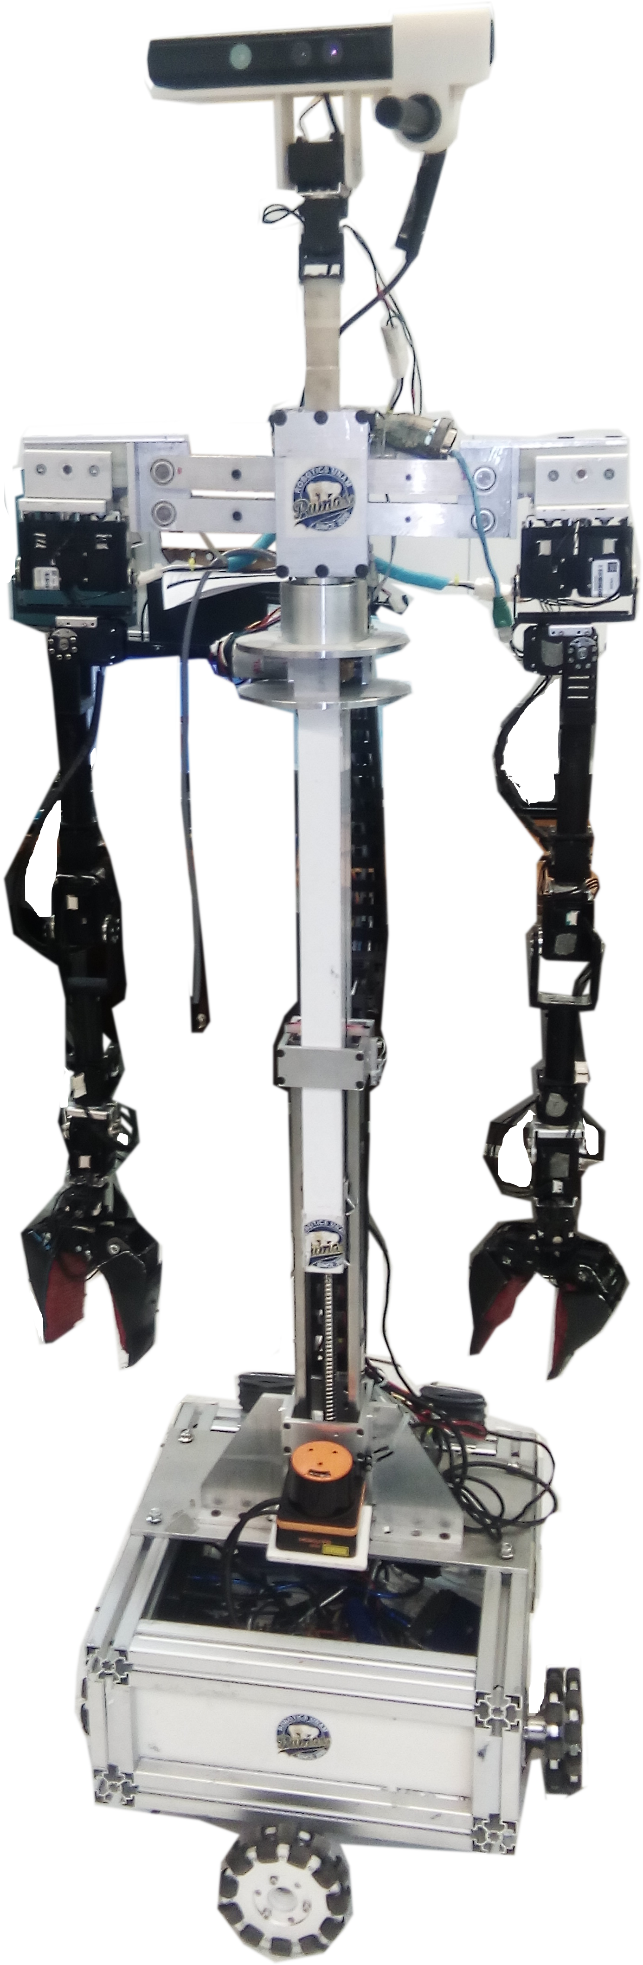
\includegraphics[width=0.7\textwidth]{Figures/Introduction/Justina.png}
\caption{El Robot Justina}
\label{fig:introduction:Justina}
\end{figure}
\pagebreak


\end{document}